% THIS IS AN EXAMPLE DOCUMENT FOR VLDB 2012
% based on ACM SIGPROC-SP.TEX VERSION 2.7
% Modified by  Gerald Weber <gerald@cs.auckland.ac.nz>
% Removed the requirement to include *bbl file in here. (AhmetSacan, Sep2012)
% Fixed the equation on page 3 to prevent line overflow. (AhmetSacan, Sep2012)

\documentclass{vldb}
\usepackage{graphicx}
\usepackage{balance}  % for  \balance command ON LAST PAGE  (only there!)
\usepackage{todonotes}
\newcommand{\systemname}{\textbf{LOKI}\xspace}
\newcommand{\sysname}{\textbf{DOKI}\xspace}



% Include information below and uncomment for camera ready
\vldbTitle{Know Your Dataset}
\vldbAuthors{Poonam Kumari, supervised by Dr. Oliver Kennedy}
\vldbDOI{https://doi.org/TBD}

\begin{document}

% ****************** TITLE ****************************************

\title{Know Your Dataset}
%{A Sample {\ttlit Proceedings of the VLDB Endowment} Paper in LaTeX
%Format\titlenote{for use with vldb.cls}}


% possible, but not really needed or used for PVLDB:
%\subtitle{[Extended Abstract]
%\titlenote{A full version of this paper is available as\textit{Author's Guide to Preparing ACM SIG Proceedings Using \LaTeX$2_\epsilon$\ and BibTeX} at \texttt{www.acm.org/eaddress.htm}}}

% ****************** AUTHORS **************************************

% You need the command \numberofauthors to handle the 'placement
% and alignment' of the authors beneath the title.
%
% For aesthetic reasons, we recommend 'three authors at a time'
% i.e. three 'name/affiliation blocks' be placed beneath the title.
%
% NOTE: You are NOT restricted in how many 'rows' of
% "name/affiliations" may appear. We just ask that you restrict
% the number of 'columns' to three.
%
% Because of the available 'opening page real-estate'
% we ask you to refrain from putting more than six authors
% (two rows with three columns) beneath the article title.
% More than six makes the first-page appear very cluttered indeed.
%
% Use the \alignauthor commands to handle the names
% and affiliations for an 'aesthetic maximum' of six authors.
% Add names, affiliations, addresses for
% the seventh etc. author(s) as the argument for the
% \additionalauthors command.
% These 'additional authors' will be output/set for you
% without further effort on your part as the last section in
% the body of your article BEFORE References or any Appendices.

\numberofauthors{1} %  in this sample file, there are a *total*
% of EIGHT authors. SIX appear on the 'first-page' (for formatting
% reasons) and the remaining two appear in the \additionalauthors section.

\author{
% You can go ahead and credit any number of authors here,
% e.g. one 'row of three' or two rows (consisting of one row of three
% and a second row of one, two or three).
%
% The command \alignauthor (no curly braces needed) should
% precede each author name, affiliation/snail-mail address and
% e-mail address. Additionally, tag each line of
% affiliation/address with \affaddr, and tag the
% e-mail address with \email.
%
% 1st. author
\alignauthor
Poonam Kumari\\
       \affaddr{Supervised by Dr. Oliver Kennedy}\\
       \affaddr{State University of New York at Buffalo, Buffalo, NY, USA}\\
       \email{\{poonamku,okennedy\}@buffalo.edu}
}
% There's nothing stopping you putting the seventh, eighth, etc.
% author on the opening page (as the 'third row') but we ask,
% for aesthetic reasons that you place these 'additional authors'
% in the \additional authors block, viz.
\additionalauthors{Additional authors: John Smith (The Th{\o}rv\"{a}ld Group, {\texttt{jsmith@affiliation.org}}), Julius P.~Kumquat
(The \raggedright{Kumquat} Consortium, {\small \texttt{jpkumquat@consortium.net}}), and Ahmet Sacan (Drexel University, {\small \texttt{ahmetdevel@gmail.com}})}
\date{30 July 1999}
% Just remember to make sure that the TOTAL number of authors
% is the number that will appear on the first page PLUS the
% number that will appear in the \additionalauthors section.


\maketitle

\begin{abstract}
It has become very easy to obtain a large dataset for experimental analysis. But most of these datasets are unlabeled or poorly labeled. Absence of labels, leads to difficulty in accessing the data.

We propose the design of a system LOKI, which would serve as a knowledge base for storing column-naming heuristics, as well as an interactive tool: the LOKI editor for populating the knowledge-base.

\todo[inline]{Poonam:paraphrase, taken from HILDA paper} 
The LOKI editor primes the knowledge base by learning from example data (e.g., from open data portals), and assists domain experts in reviewing and refining the resulting heuristic naming schemes. We identify specific issues arising from training and show how the LOKI editor streamlines the process of manually repairing these issues.

\end{abstract}

\section{Motivation}
Big datasets are available in abundance and are being used by data scientists and database community for research purpose. These datasets are often curated, analyzed and forgotten without any documentation about the dataset itself. We propose to end this cycle by designing a system with a central goal of inferring column names by creating a knowledge base, which would store a collection of rules and column-naming heuristics (LOKI: Label Once and Keep It), as well as help start the documentation for a dataset (DOKI: Document Once and Keep It).

So when presented a new dataset our system would start with creating LOKI and DOKI. LOKI would help an analyst in inferring the column names for new datasets and using DOKI the analyst can start documenting the dataset. Apart from creating a knowledge base LOKI also provides an interactive tool for populating the knowledge base.


\section{Research Questions}
Given a dataset the user wants to analyze, the system performs two steps (1) create LOKI and (2) create DOKI. Once a dataset is documented the analyst can save the documentation for future use.  

The first step is to create LOKI which helps in streamlining the process of developing schemas for unlabeled or poorly labeled datasets. LOKI provides users with two modes of interaction: (1) A labeling interface that assists users in assigning names to existing columns of data, and (2) A discovery interface that helps users to search for columns representing particular concepts of interest. These interfaces are supported by a knowledge-base that combines expert-provided heuristics, learned characteristics, as well as historical feedback gathered from users about already-loaded datasets. Once the user has labeled or discovered a sufficient set of columns, LOKI generates appropriate data loading/initialization code (e.g., a CREATE TABLE or Spark DataFrame initializer).

Once LOKI is created, the next step is to create DOKI. ~\ref{fig:DOKI} illustrates the different components of dataset that DOKI helps store.

\begin{figure}[h]
	\centering
	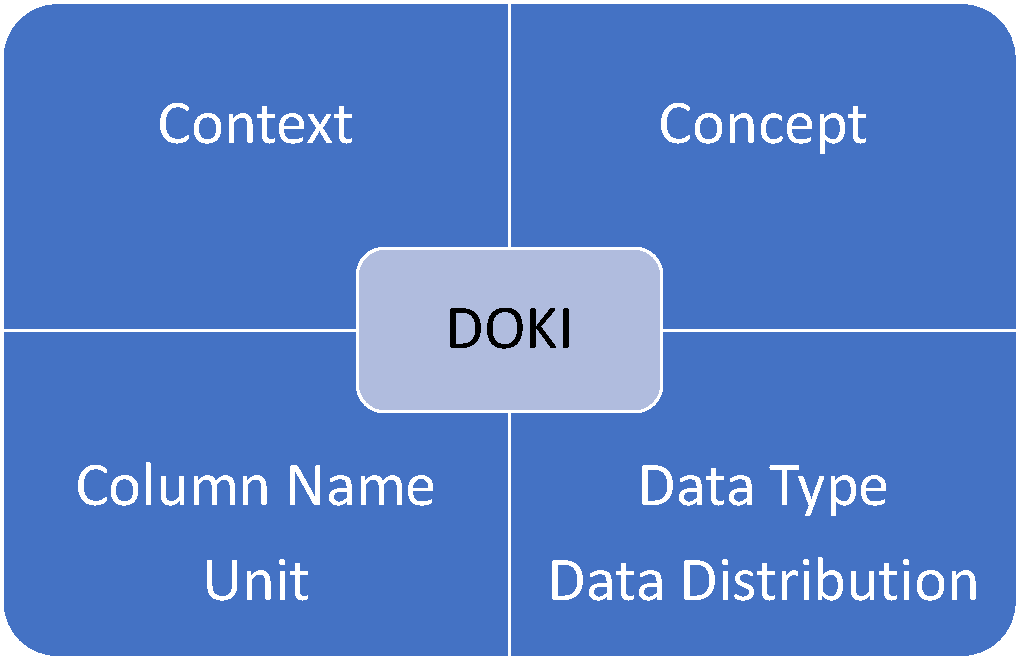
\includegraphics[width=0.8\columnwidth]{graphics/DOKI.pdf}
	\caption{Document Once and Keep It overview}
	\label{fig:DOKI}
	\vspace*{-1mm}
\end{figure}

Context stores the details of the domain to which the dataset belongs. Concepts correspond to names. Since the same name may be used in different contexts, multiple concepts can use the same column name. Similarly, a single concept may be associated with multiple names.
Unit refers to the mathematical unit associated with a column. e.g. Kilogram, Hectares, etc. Name stores the column name. Type of data present in the dataset whether it is numerical, categorical, datetime etc are stored as data type. Data distribution refers to the distribution that best describes a column. e.g Normal, uniform, zipfian etc.

\newtheorem{exmp}{Example}[section]
\begin{exmp}
	This is an example
\end{exmp}

\begin{center}
	\begin{tabular}{||c c c c||} 
		\hline
		Col1 & Col2 & Col2 & Col3 \\ [0.5ex] 
		\hline\hline
		1 & 6 & 87837 & 787 \\ 
		\hline
		2 & 7 & 78 & 5415 \\
		\hline
		3 & 545 & 778 & 7507 \\
		\hline
		4 & 545 & 18744 & 7560 \\
		\hline
		5 & 88 & 788 & 6344 \\ [1ex] 
		\hline
	\end{tabular}
\end{center}

analyst can reuse it without any difficulty. The analyst does not have to document the dataset again, and is well versed with the dataset through the information stored in knowledge base(data type, data distribution). The knowledge base would store expert inputs and feedback \todo[inline]{Explain.What do you mean by expert inputs and feedback?} and also help the analyst in identifying schema names for new datasets. The system named LOKI serves as a knowledge base and an interactive tool for populating the knowledge base. When a user first points LOKI at a new tabular data set, LOKI proposes a schema \todo[inline]{just schema?} for it. It then collects feedback, both learning and also preserving schema metadata for later use.


\todo[inline]{Poonam:rewrite, taken from HILDA paper} 
In short, LOKI will allow users to assemble schemas on-demand, both (re-)discovering and incrementally refining schema definitions in response to changing data needs. 

However, to accomplish this, we first need a knowledge-base of heuristics, domain knowledge, and dirty tricks. In principle, we might implement such a knowledge base as a neural network, train it on example data, and use it to suggest schemas. However, this approach suffers from a host of limitations:
(1) Lack of generality: A neural network tuned for use with one
type of training data may need to be retuned for other scenarios.
(2) Lack of extensibility: Adding new training data or knowledge network misclassifies a column name, it can be hard to debug and
refine the result. Instead, we opt for an interactive approach. We
present the LOKI knowledge-base, a flexible, extensible infrastructure
for collecting schema-naming heuristics.We show how simple,
efficient off-the-shelf techniques can be used to quickly prime the
knowledge-base using example data. Then, we introduce an interactive
editor that we are designing as part of LOKI to allow domain
experts to refine the knowledge-base. In particular, we focus on our
preliminary work to streamline manual refinement of knowledge
learned from one type of example data. We show how, the editor
can be used to help experts to quickly identify and resolve errors
and ambiguity in the LOKI knowledge-base.
Concretely, the contributions of this paper include: (1) We introduce
LOKI in Section 2 and detail the structure of its knowledge-
base in Section 3. (2) We illustrate how the LOKI editor
pre-populates the knowledge-base by learning from example data
in Section 4. (3)We identify specific errors that arise in the training
process and showhowthe LOKI editor facilitates efficient detection
and manual repair of the error in Section 5.

Documentation would consist of storing the following information about the dataset:

\begin{itemize}
	\item Context: Domain to which the column belongs.
	\item Concept: Noun that describes a column.
	\item Unit: Mathematical unit associated with the column. e.g. Kilogram, Hectares, etc.
	\item Name: String name associated with the column. e.g. A column containing patients blood pressure might be named BP.
	\item Signature: Parameters used to describe a column. It is a combination of context, Range, Distribution, set of values and the type of data.
	\item Column: 
	\item Data type:
	\item Data distribution:
\end{itemize}

\subsection{Challenges}
\begin{enumerate}
	\item Column might match on multiple signatures
	\item Similar concepts with different signatures
	\item Similar signatures for different concepts
	\item Insufficient signal for signature based matching.
	->types of signature insufficient
	\item different signatures combine differently to id concepts
	\item performance
\end{enumerate}

\section{Related Work}
\todo[inline]{Poonam:rewrite, taken from HILDA paper} 
Data distributions have been used for similar purposes in other work.  
For example GestureQuery~\cite{nandi2013gestural} uses data similarity between two attributes to select candidate attributes for an equi-join.  
To maximize the join arity, the system counts the number of times each value from one attribute appears in the other and a histogram is constructed from the counts for all of the values.

Wrangler \cite{kandel2011wrangler} and Potter's wheel \cite{raman2001potter} detect data domains through inclusion functions (e.g. regular expressions).
Wrangler in particular infers the data type of a column and highlights errors based on inconsistent data types. 
Wrangler also has several operators like split and unfold that create new columns.
The split operator decomposes composite data values into component distributions.  
The unfold operator reverses a table pivot, collapsing data laid out as key-value pairs into columns.  
A useful application of the LOKI knowledge-base that we hope to explore in future work is using it to detect opportunities for applying such operators.

An orthogonal approach to modeling and matching columns is to use ontologies, which express entities, facts, relations between facts and properties of relations
Ontologies like Yago \cite{fabian2007yago} could be used to identify semantic properties that relate columns.

A data summary called the data describer is used in \cite{ping2017datasynthesizer}. The data types, correlations and distributions of the attributes in a private dataset are listed. Each attribute is categorized into either numerical or non-numerical. If non-numerical attribute cannot be parsed as datetime then it is considered to be a string.

Data describer takes in a CSV file and infers the data types and domains. The attribute datatypes are parsed as numerical, datetime or string. We are inferring the datatypes as well. When run in correlated attribute mode, data describer provides corelation between attributes. We could use this functionality in LOKI.
% \todo{What exactly is the purpose of the data describer.  How is it used?  How do its goals differ from ours, and what are the implications on its design?} 

PADS \cite{fisher2005pads} helps users to understand the layout and meaning of data by designing syntactic descriptions of the data.
Based on the syntax, accumulators track the number of good values, the number of bad values, and the distribution of legal values.
This technique could be used in LOKI to help capture expert knowledge.

There is an increasing number of datasets in which well-structured attributes
(with or without a name) can be identified, each containing a set of values called a domain. There is lack of schema description in most of the datasets.
LSH Ensemble is used in \cite{zhu2016lsh} to find domains that maximally contain a query dataset, which can help to find datasets that best augment a given set of data.

\section{Experiments}
\todo[inline]{Poonam:rewrite, taken from HILDA paper} 
Describe how KB was created for datasets. System design from HILDA paper

\section{Research Plan}
We plan several extensions as future work focused on building and
refining a knowledge-base for storing column-naming heuristics.
• Use of contextual information: Contextual information
such as ontologies, units and data domains could be used to augment
the LOKI knowledge base (KB). We could use a network of
semantic relations such as BabelNet strengthen data models for
training the KB as well as providing curation recommendations
to experts. [2] • Recommendation of columns for query: Concepts
in the KB could be used to recommend columns that could be
in a query based on the columns that are already present. • Smarter
Matchers:We would develop matchers which regocognize a wider
spectrum of data. For example, regular expression matchers could
be used to detect geolocation data. Matchers which can identify
synonymous labels could help experts in the curation process.

\todo[inline]{Poonam:for reference} 
To overcome the assumptions and limitations of the current
framework we propose the following research plan: (1)
We want to generalize candidate questions to include nonboolean
atoms. In this way, same incomplete data in different
candidate questions can be confirmed in one confirmation
round. (2) The current framework assumes the probability
distributions for incomplete data are given. However,
this is not always feasible. We want to make use of the existing
reliable data to estimate the probability distribution of
incomplete data. (3) In many domains, there exist models
that can be utilized to increase query result accuracy without
consulting users. Currently, in the UDLM component,
we mainly utilized the user-defined models to preprocess incomplete
data at no cost. We want to explore how to learn
models from system-user interactions. For instance, in data
integration, possible schema matches are candidate models,
one of which is a correct match. We can treat each candidate
model as probabilistically related to the real model. We can
integrate these candidate models with our current framework
and adjust the confidence of a model on confirmation.
The probability will converge on true model. This learned
model will be utilized adaptively in subsequent queries. (4)
Our current framework considers user feedback is always
correct. However, humans may make mistakes. In crowdsourcing,
humans may provide incorrect answers to tasks
accidentally or on purpose. In medical expert systems, user
feedback is obtained based on test results by machines. The
test results may not be 100% accurate. We want to build
a user profile to record the credibility of user feedback. We
need to decide how to integrate this profile with our frame work and based on the correctness of the decisions made


\section{Conclusion}
\todo[inline]{Poonam:for reference} 
This paper proposes the design of a system which would help build a knowledge base along with an interactive tool for populating the knowledge base. 
\todo[inline]{Mention Query model?}


%\end{document}  % This is where a 'short' article might terminate

% ensure same length columns on last page (might need two sub-sequent latex runs)
\balance

%ACKNOWLEDGMENTS are optional
\section{Acknowledgments}
This work was supported by NSF Awards IIS-1750460, ACI-1640864
and by a gift from Oracle. The conclusions and opinions in this
work are solely those of the authors and do not represent the views
of the National Science Foundation or Oracle.


% The following two commands are all you need in the
% initial runs of your .tex file to
% produce the bibliography for the citations in your paper.
\bibliographystyle{abbrv}
\bibliography{vldb_sample}  % vldb_sample.bib is the name of the Bibliography in this case
% You must have a proper ".bib" file
%  and remember to run:
% latex bibtex latex latex
% to resolve all references

%APPENDIX is optional.
% ****************** APPENDIX **************************************
% Example of an appendix; typically would start on a new page
%pagebreak



\end{document}
